%https://tex.stackexchange.com/questions/584590/tikz-double-sideband-dsb-spectrum
\documentclass[tikz,border=3.14159mm,subpreambles=true]{standalone}

\providecommand{\DSBA}[5]{
    \def\xa{#2} \def\ya{0}
    \def\xb{\xa/2} \def\yb{#5}
    \def\xc{0} \def\yc{#5}
    \def\tang{\xa/3}
    %   
    \def\curve{
            (#1-\xa,\ya) .. controls ++ (2*\tang,0) and ++ (-\tang,0) ..
            (#1-\xb,\yb) .. controls ++ (.5*\tang,0) and ++ (-\tang,0) ..
            (#1,\yc) .. controls ++ (\tang,0) and ++ (-.5*\tang,0) ..
            (#1+\xb,\yb) .. controls ++ (\tang,0) and ++ (-2*\tang,0) ..
            (#1+\xa,\ya)
            }
    \path[fill=#3!#4] (#1-\xa,0) -- \curve -- (#1+\xa,0) -- cycle;
    \draw  \curve;
    }
\providecommand{\DSBB}[5]{
    \def\xa{#2} \def\ya{0}
    \def\xb{\xa/2} \def\yb{#5}
    \def\xc{0} \def\yc{#5}
    \def\tang{\xa/3}
    %   
    \def\curve{
            (#1-\xa,\ya) .. controls ++ (2*\tang,0) and ++ (-\tang,0) ..
            (#1-\xb,\yb) .. controls ++ (.5*\tang,0) and ++ (-\tang,0) ..
            (#1,\yc) .. controls ++ (\tang,0) and ++ (-.5*\tang,0) ..
            (#1+\xb,\yb) .. controls ++ (\tang,0) and ++ (-2*\tang,0) ..
            (#1+\xa,\ya)
            }
    \path[fill=#3!#4] (#1-\xa,0) -- \curve -- (#1+\xa,0) -- cycle;
    \draw[color=#3!#4]  \curve;
    }


        
\begin{document}
    
    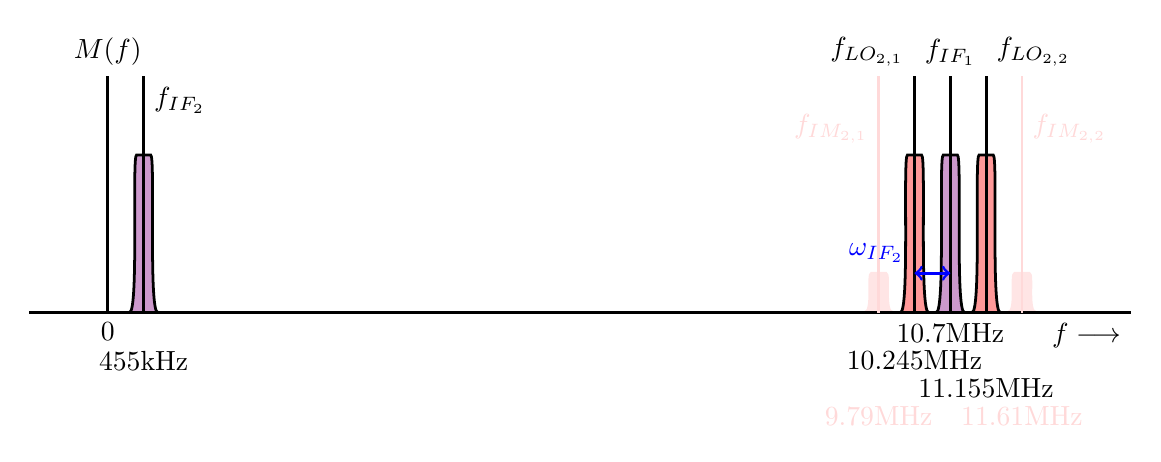
\begin{tikzpicture}[
        line width=1pt,
        sb/.style={text width=1.5cm, align=center,inner sep=0pt}]
        
    \DSBA{10.7}{0.18}{violet}{40}{2}
    \DSBA{10.245}{0.18}{red}{40}{2}
    \DSBA{11.155}{0.18}{red}{40}{2}
    \DSBA{0.455}{0.18}{violet}{40}{2}
    \DSBB{9.79}{0.18}{pink}{40}{0.5}
    \DSBB{11.61}{0.18}{pink}{40}{0.5}
    \draw   (-1,0) -- (13,0) node [below left] {$f \longrightarrow$}
            (0,0) node[below] {0} --++ (0,3) node [above] {$M(f)$}
            (10.7,0) node[below] {10.7MHz} --++ (0,3) node [above] {$f_{IF_1}$}
            (10.245,0) node[below,yshift=-10] {10.245MHz} --++ (0,3) node [above left] {$f_{LO_{2,1}}$}
            (11.155,0) node[below,yshift=-20] {11.155MHz} --++ (0,3) node [above right] {$f_{LO_{2,2}}$}
            (0.455,0) node[below,yshift=-10] {455kHz} --++ (0,3) node [below right] {$f_{IF_2}$};
    \draw[<->, color=blue] (10.245,0.5)--(10.7,0.5);
    \draw[color=pink!60] (9.79,0) node[below,yshift=-30,color=pink!60] {9.79MHz} --++ (0,3) node [below left,yshift=-10,color=pink!60] {$f_{IM_{2,1}}$}
    (11.61,0) node[below,yshift=-30,color=pink!60] {11.61MHz} --++ (0,3) node [below right,yshift=-10,color=pink!60] {$f_{IM_{2,2}}$};
    \node[align=center, above left, color=blue] at (10.245,0.5) {$\omega_{IF_2}$};
                
    \end{tikzpicture}
\end{document}